 \documentclass[10pt, handout]{beamer}

\usetheme[progressbar=frametitle]{metropolis}
\usepackage{appendixnumberbeamer}
\usetikzlibrary{arrows.meta, positioning, quotes}
\usepackage{enumitem}

\usepackage{booktabs}
\usepackage[scale=2]{ccicons}

\usepackage{pgfplots}
\usepgfplotslibrary{dateplot}

\usepackage{xspace}
\newcommand{\themename}{\textbf{\textsc{metropolis}}\xspace}

\title{Machine Learning I}
\subtitle{Lecture 1 - Introduction to Machine Learning}
% \date{\today}
\date{}
\author{Nathaniel Bade}
\institute{Northeastern University Department of Mathematics}
% \titlegraphic{\hfill\includegraphics[height=1.5cm]{logo.pdf}}

\begin{document}

\maketitle

\begin{frame}{Table of contents}
  \setbeamertemplate{section in toc}[sections numbered]
  \tableofcontents[hideallsubsections]
\end{frame}



\section{What is Machine Learning?} %ML vs Statistics vs Probabiltiy



\begin{frame}[t]{Statistical Modeling}
  \begin{minipage}[t][0.5\textheight][t]{\textwidth}
    \centering
     \includegraphics[height=0.5\textheight]{MRIScans.png}
  \end{minipage}
  \vfill
  \begin{minipage}[t][0.5\textheight][t]{\textwidth}
In the MRI scans above (from the OASIS 1 data set), the top three images come from a patient who has not been diagnosed with dementia. The bottom image come from a patient who has been diagnosed with severe dementia. Human doctors looking at these images wouldn't expect to be able to detect any difference between the brains, but maybe computational methods can do better?
  \end{minipage}
\end{frame}



\begin{frame}[t]{Statistical Modeling}
  \begin{minipage}[t][0.5\textheight][t]{\textwidth}
    \centering
     \includegraphics[height=0.5\textheight]{MRIScans.png}
  \end{minipage}
  \vfill
  \begin{minipage}[t][0.5\textheight][t]{\textwidth}
But how can we discover how this data is organized? Is dementia normally distributed? \pause Each MRI is contains 6,443,008 pixels and so mathematically is an element of $\mathbb{R}^{6443008}$, can we hope to write down a distribution on this space?
  \end{minipage}
\end{frame}


\begin{frame}[t]{Statistical Modeling}
  \begin{minipage}[t][0.5\textheight][t]{\textwidth}
    \centering
     \includegraphics[height=0.5\textheight]{MRIScans.png}
  \end{minipage}
  \vfill
  \begin{minipage}[t][0.5\textheight][t]{\textwidth}
\textbf{Machine learning} is discipline that deals with fitting mathematical models to intractable distributions of data. In recent years, computational increases have enabled us to attack higher and higher dimensional  problems, sometimes with very little data, sometimes with terabytes of information. 
  \end{minipage}
\end{frame}



\begin{frame}[t]{Statistical Modeling}
  \begin{minipage}[t][0.5\textheight][t]{\textwidth}
    \centering
     \includegraphics[height=0.5\textheight]{MRIScans.png}
  \end{minipage}
  \vfill
  \begin{minipage}[t][0.5\textheight][t]{\textwidth}
In low dimensions and with sparse data, empirical reasoning often leads to careful and informative models. In the high dimensional world of machine learning, a suite of so called ``black box'' models has been developed that can be tuned to a wide variety of problems. Some of these models are straightforward, like linear regression, but some like neural networks may contain millions of variables, and it is still an open question as to what structure exactly they are probing. 
  \end{minipage}
\end{frame}


\begin{frame}[t]{Statistical Modeling}
In this course, we will learn both the mathematical and the implementation of the core machine learning methods: Linear models, linear basis fitting, neural networks, decision trees and cluster analysis. Over the course of the semester we will analyze and implement all of the mathematical pieces that go into a machine learning algorithm, and show how they fit into the physical implementation of a machine learning project. Along the way, we will talk about how to combine and ensemble train models, boot strap data and use machine learning to learn which algorithm to use.

We will finish the semester by putting machine learning in it's proper mathematical context, discussing learnability, the partially approximately correct learning framework, the No Free Lunch Theorem, and VC Dimension. 

Throughout the course, we will be working on a large scale machine learning project with the aim to bring all of our methods and methodologies to bear on solving hard, real world problems. 
\end{frame}





\section{Statistical Learning Theory}


\begin{frame}[fragile]{Statistical Learning Theory}
This course will use \textbf{statistical learning theory} to understand the mathematical aspects of \textbf{machine learning}. Machine learning is the process of fitting the parameters of a model to a given set of data.

\textbf{Statistical learning theory} is roughly about understanding how much data is required to make predictions using a fit model to a certain degree of accuracy. We will first understand some theoretical aspects of the theory, and then move to practical implementation using Python.
\end{frame}


\begin{frame}[t]{Statistical Modeling}
  \begin{minipage}[t][0.5\textheight][t]{\textwidth}
    \centering
     \includegraphics[height=0.5\textheight]{L1StatsModel1.png}
  \end{minipage}
  \vfill
  \begin{minipage}[t][0.5\textheight][t]{\textwidth}
  \textbf{Example:} Student height: In a school, students ages $a_i$ are uniformly distributed between ages 6 and 11. We can fit a mathematical function to this data to model it, and then use the function to predict the heights of a new set of students using the data. 
  \end{minipage}
\end{frame}


\begin{frame}[t]{Statistical Modeling}
  \begin{minipage}[t][0.5\textheight][t]{\textwidth}
    \centering
     \includegraphics[height=0.5\textheight]{L1StatsModel1.png}
  \end{minipage}
  \vfill
  \begin{minipage}[t][0.5\textheight][t]{\textwidth}
There are many choices that go into such a modeling project: Should we use a \textbf{linear} model or a \textbf{polynomial} model? \pause For a linear model $h_i = c \, a_i + d$, how do we pick  $c$ and $d$ based on the data? \pause Once we fit the data, where is it reasonable to use the model? \pause How much data do we need to get an accurate answer?
  \end{minipage}
\end{frame}




\begin{frame}[fragile]{Statistical Modeling}
Formally, \textbf{Statistical modeling} starts with a sample space $S$, with data points distributed by an (unknown) probability distribution on $S$. We then posit a mathematical model $F_\theta(X)$ depending on parameters $\theta$ to generate estimates about the likelihood of observed data. \pause

In the previous example, if $X\in \mathbb{R}$ is age and $Y\in \mathbb{R}$ is height, and we fit some function $f_B:X\to Y$ to give a labeling of data. By adding in a random variable $\epsilon$ with variance $\sigma^2$, we can write the  statistical model

\begin{center}
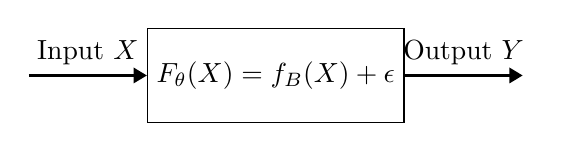
\begin{tikzpicture}[
 	node distance=5mm and 30mm,
	box/.style = {draw, minimum height=12mm, align=center},
	sx+/.style = {xshift= 15mm}, 
	sx-/.style = {xshift=-15mm},
	every edge quotes/.style = {align=center}
     ]
		\node (n1) [box] {$F_\theta(X) = f_B(X) + \epsilon$};              
%
		\draw[thick,-Triangle]
		([sx-] n1.west) to [above,"Input $X$"] (n1.west);
%
		\draw[thick,-Triangle]
		(n1.east) to [above,"Output $Y$"] ([sx+] n1.east);
\end{tikzpicture}
\end{center}
We then pick $\theta$ to maximize the probability, or likelihood, the the datapoints we observe are drawn from the model. In the above, $\theta = (B, \sigma^2)$ parameterize both the choices in our model $\theta$, and the choices about the noise $\sigma^2$. 
\end{frame}





\begin{frame}[t]{Statistical Modeling}
  \begin{minipage}[t][0.5\textheight][t]{\textwidth}
    \centering
     \includegraphics[height=0.5\textheight]{L1StatsModel2.png}
  \end{minipage}
  \vfill
  \begin{minipage}[t][0.5\textheight][t]{\textwidth}
We might then predict height $h_i$ of child $i$ via their age $a_i$, using the model
$$
h_i = b_0 + b_1 a_i + \epsilon_i\,.
$$
We include a stochastic variable $\epsilon_i$ since $h_i$ must fit all the data. To do statistical inference, we make the assumption that $\epsilon_i$ is Gaussian. 
  \end{minipage}
\end{frame}




\begin{frame}[t]{Statistical Modeling}
  \begin{minipage}[t][0.5\textheight][t]{\textwidth}
    \centering
     \includegraphics[height=0.5\textheight]{L1StatsModel3.png}
  \end{minipage}
  \vfill
  \begin{minipage}[t][0.5\textheight][t]{\textwidth}
\begin{flalign*}
\boxed{\,\,Model:\,}&&h_i = b_0 + b_1 a_i + \epsilon_i&&&&&
\end{flalign*}
\textbf{Sample space:} $S = [6,11]\times \mathbb{R}^+$ all possible pairs $(a,h)$. 

\textbf{Parameters:} $\theta = (\sigma^2, b_0,b_1)$. Each triple of values defines a model distribution $P_\theta$ on $X$. 
\pause
$P$ is the set of all such distributions. 
\end{minipage}
\end{frame}


\begin{frame}[t]{Statistical Modeling}
  \begin{minipage}[t][0.5\textheight][t]{\textwidth}
    \centering
     \includegraphics[height=0.5\textheight]{L1StatsModel4.png}
  \end{minipage}
  \vfill
  \begin{minipage}[t][0.5\textheight][t]{\textwidth}
\begin{flalign*}
\boxed{\,\,Model:\,}&&h_i = b_0 + b_1 a_i + \epsilon_i&&&&&
\end{flalign*}
\textbf{Sample space:} $X = [6,11]\times \mathbb{R}^+$ all possible pairs $(a,h)$. 

\textbf{Parameters:} $\theta = (\sigma^2_\epsilon, b_0,b_1)$. Each triple of values defines a distribution $P_\theta$ on $X$. 
$P$ is the set of all such distributions. 
\end{minipage}
\end{frame}




\begin{frame}[fragile]{Machine Learning vs Statistics}
\textbf{Machine learning} is used in problems where the underlying distributions are unknown or unknowable. Typical examples include image classification, voice recognition, or gene expression. 

\begin{center}
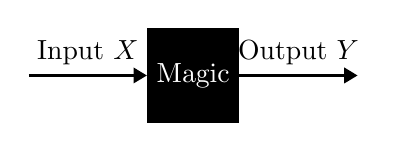
\begin{tikzpicture}[
 	node distance=5mm and 30mm,
	box/.style = {draw, minimum height=12mm, align=center},
	sx+/.style = {xshift= 15mm}, 
	sx-/.style = {xshift=-15mm},
	every edge quotes/.style = {align=center}
     ]
		\node[fill=black,text=white] (n1) [box] {Magic};              
%
		\draw[thick,-Triangle]
		([sx-] n1.west) to [above,"Input $X$"] (n1.west);
%
		\draw[thick,-Triangle]
		(n1.east) to [above,"Output $Y$"] ([sx+] n1.east);
\end{tikzpicture}
\end{center}
Machine learning uses black-box methods that strive for accuracy regardless of the underlying distribution. 
\pause

\textbf{Main Question:} For a given class of models, how many data points do we need in order to be certain (probabilistically) that the error in our model is small \textit{no matter what the underlying distribution}.
\end{frame}






\begin{frame}[fragile]{Machine Learning Examples: Cats and Dogs}
\includegraphics[width=10.8cm]{L1DogCat.png}
\textbf{Example:} 
In image classification, input $X = \mathbb{R}^{3\times 100\times 200}$ and output $Y = \{\text{"Dog"},\text{"Cat"}\}$. \pause 

How do we find the distribution on the state space $S = X\times Y$?
\end{frame}




\begin{frame}[fragile]{Machine Learning Examples: Computer Vision}
\includegraphics[width=10.8cm]{L1MNIST.png}
\textbf{Example:} 
For multilable classification, input $X = \mathbb{R}^{20\times 20}$ and output $Y = \{0,1,2,3,4,5,6,7,8,9\}$. Above is the famous MNIST data set of handwritten numbers. 
\end{frame}






\begin{frame}[fragile]{Machine Learning Examples: Iris Classification}
\includegraphics[width=10.8cm]{L1IrisClass.png}

\begin{tabular}{llcll}
\textbf{Sepal Length} & \textbf{Sepal Width} & \textbf{Petal Length} & \textbf{Petal Width} & \textbf{Species}\\ \hline
 	5.1 &	3.5 &	1.4 &	0.2 &	I. Setosa         \\ \hline
7.0 	& 3.2  &	4.7 &	1.4 &	I. Versicolor         \\ \hline
&&$\vdots$
\end{tabular}


\textbf{Example:} Classification by Attributes: 
Input is $X = \mathbb{R}^4$ and output is a finite set $\mathcal{G} = \{\text{Virginica, Setosa, Versicolor}\}.$
\end{frame}







\begin{frame}[fragile]{Machine Learning Examples: Market Segmentation}
\begin{center}
\includegraphics[width=8cm]{L1Cluster.png}
\end{center}
\begin{tabular}{llcll}
\textbf{UserID} & \textbf{Products} \\ \hline
0x131432 & \{"Leather Hat", "Dvvorsh Black Belt", "Dukes Hat Polish",...\}  \\ \hline
0x152341 & \{"Tinga XL Beach Towel", "Speco Meat Thermometer",...\}     \\ \hline
&&$\vdots$
\end{tabular}


\textbf{Example:} Clustering: 
Input is $X = \mathbb{P}(\{\text{All Products}\})$, the powerset of the set of all products. 
\end{frame}


\begin{frame}[fragile]{Machine Learning vs Statistics}
\textbf{Machine learning} is used in problems where the underlying distributions are unknown or unknowable.

\begin{center}
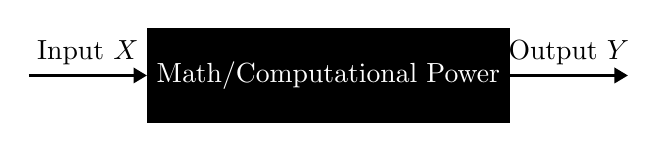
\begin{tikzpicture}[
 	node distance=5mm and 30mm,
	box/.style = {draw, minimum height=12mm, align=center},
	sx+/.style = {xshift= 15mm}, 
	sx-/.style = {xshift=-15mm},
	every edge quotes/.style = {align=center}
     ]
		\node[fill=black,text=white] (n1) [box] {Math/Computational Power};              
%
		\draw[thick,-Triangle]
		([sx-] n1.west) to [above,"Input $X$"] (n1.west);
%
		\draw[thick,-Triangle]
		(n1.east) to [above,"Output $Y$"] ([sx+] n1.east);
\end{tikzpicture}
\end{center}

\textbf{Main Question:} For a given class of models, how many data points do we need in order to be certain (probabilistically) that the error in our model is small \textit{no matter what the underlying distribution}.
\end{frame}







\section{Terminology and Notation}




\begin{frame}[fragile]{Two Types of Machine Learning}

\textbf{Supervised Learning:} Given a sample set of \textit{labeled} data, can we predict the labels on new unlabeled data from the same domain?

\textit{Examples: Image classification, classification by features.}\vspace{3em}

\textbf{Unsupervised Learning:} Given a set of \textit{unlabeled} data, can we find structure within the data? 

\textit{Examples: Clustering, dimensional reduction.}
\end{frame}



\begin{frame}[fragile]{Variable Types}
There are two large families of variable types:\pause

\textbf{Qualitative Variables:} Variables that only take discrete values, usually in a set of descriptive \textbf{classes}. Also called \textbf{categorical} or \textbf{discrete} variables, or \textbf{factors}. There could be no additional ordering or structure on the classes.

\textit{Examples: Iris name, "Cat" or "Dog", items purchased, the integers 0 to 9 in MNIST.}

\vspace{3em}\pause


\textbf{Quantitative Variables:} Variables that take quantitative values, with some values larger than others and close values designating similar characteristics. Also called \textbf{numerical}.


\textit{Examples: Body temperature, grayscale value of a pixel, stem length, height.}\vspace{3em}
\end{frame}



\begin{frame}[fragile]{Regression}


\textbf{Regression analysis} is a set of procedures for estimating the relationships between independent variables (inputs) and dependent variables (outputs).

In ESL, \textbf{regression} specifically refers to prediction when the outputs are quantitative. If the outputs are qualitative, this is referred to as \textbf{classification}.

In UML, \textbf{regression} refers to any \textit{functional} relationship between the domain of the inputs $X$ and the range of the outputs $Y$, regardless of variable type.

This ambiguity can be found throughout the field. 
\end{frame}




\begin{frame}[fragile]{Inputs and Output}
\begin{center}
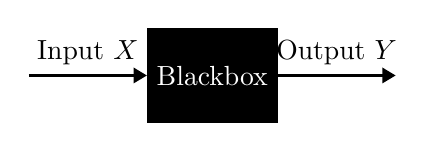
\begin{tikzpicture}[
 	node distance=5mm and 30mm,
	box/.style = {draw, minimum height=12mm, align=center},
	sx+/.style = {xshift= 15mm}, 
	sx-/.style = {xshift=-15mm},
	every edge quotes/.style = {align=center}
     ]
		\node[fill=black,text=white] (n1) [box] {Blackbox};              
%
		\draw[thick,-Triangle]
		([sx-] n1.west) to [above,"Input $X$"] (n1.west);
%
		\draw[thick,-Triangle]
		(n1.east) to [above,"Output $Y$"] ([sx+] n1.east);
\end{tikzpicture}
\end{center}

\textbf{Input variables} will be denoted by $X$. If $X$ is a vector, its components will be $X_j$. The domain of these variables will be denoted $\mathcal{X}$. 

In general, \textbf{output variables} will be denoted by $Y$. If we need to distinguish that the output is qualitative we will denote it by $G$. The domain of these variables will be $\mathcal{Y}$ and $\mathcal{G}$ respectively. 

We use uppercase $X$, $Y$, $G$ to refer to generic aspects of the variable and lowercase to denote observed values. For example, $x_i$ denotes the $i$'th \textit{observed} value of $X$ and is a vector if $X$ is. 

All vectors are assumed to be column vectors.
\end{frame}




\begin{frame}[fragile]{Inputs and Output}
\begin{center}
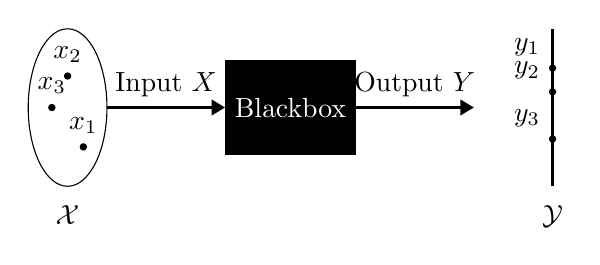
\begin{tikzpicture}[
 	node distance=5mm and 30mm,
	box/.style = {draw, minimum height=12mm, align=center},
	sx+/.style = {xshift= 15mm}, 
	sx-/.style = {xshift=-15mm},
	sx--/.style = {xshift=-20mm},
	sX--/.style = {xshift=-20mm,yshift=-1cm},
	sY--/.style = {xshift=25mm,yshift=-1cm},
	sx1--/.style = {xshift=-18mm,yshift=-5mm,},
	sx2--/.style = {xshift=-20mm,yshift=4mm},
	sx3--/.style = {xshift=-22mm,yshift=0mm},
	sxt++/.style = {xshift=25mm,yshift=1cm},
	sxb++/.style = {xshift=25mm,yshift=-1cm},
	sy1/.style = {xshift=25mm,yshift=5mm,},
	sy2/.style = {xshift=25mm,yshift=2mm},
	sy3/.style = {xshift=25mm,yshift=-4mm},
	every edge quotes/.style = {align=center},
	mycirc/.style={circle,fill=black, scale=.01cm}
     ]
		\node[fill=black,text=white] (n1) [box] {Blackbox};              
%
		\draw[thick,-Triangle]
		([sx-] n1.west) to [above,"Input $X$"] (n1.west);
%
		\draw[thick,-Triangle]
		(n1.east) to [above,"Output $Y$"] ([sx+] n1.east);
%
		\draw ([sx--] n1.west) ellipse (.5cm and 1cm);
		\node [mycirc,label=above:{$x_1$}] at ([sx1--] n1.west) {};
		\node [mycirc,label=above:{$x_2$}] at ([sx2--] n1.west) {};
		\node [mycirc,label=above:{$x_3$}] at ([sx3--] n1.west) {};
		\node [label=below:{$\mathcal{X}$}] at ([sX--] n1.west) {};
%
		\draw[thick,black] ([sxt++] n1.east) to ([sxb++] n1.east) ;
		\node [mycirc,label=above left:{$y_1$}] at ([sy1] n1.east) {};
		\node [mycirc,label=above left:{$y_2$}] at ([sy2] n1.east) {};
		\node [mycirc,label=above left:{$y_3$}] at ([sy3] n1.east) {};
		\node [label=below:{$\mathcal{Y}$}] at ([sY--] n1.east) {};
\end{tikzpicture}
\end{center}

We assume that we have access to a set of $N$ observations $(x_i,y_i)\in \mathcal{X}\times\mathcal{Y}$, for $i=1,\ldots, N$. This set of observations is called the \textbf{training set} or \textbf{training data}.

$N$ will almost always denote the number of observed points (data points in the training set).


\end{frame}


\begin{frame}[fragile]{Inputs and Output}
\begin{center}
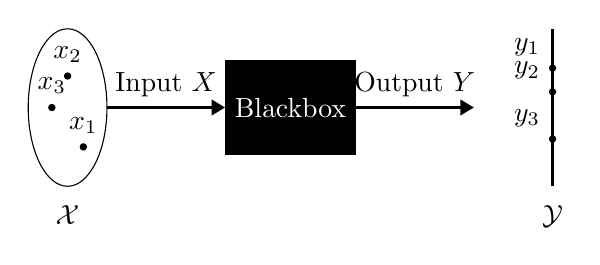
\begin{tikzpicture}[
 	node distance=5mm and 30mm,
	box/.style = {draw, minimum height=12mm, align=center},
	sx+/.style = {xshift= 15mm}, 
	sx-/.style = {xshift=-15mm},
	sx--/.style = {xshift=-20mm},
	sX--/.style = {xshift=-20mm,yshift=-1cm},
	sY--/.style = {xshift=25mm,yshift=-1cm},
	sx1--/.style = {xshift=-18mm,yshift=-5mm,},
	sx2--/.style = {xshift=-20mm,yshift=4mm},
	sx3--/.style = {xshift=-22mm,yshift=0mm},
	sxt++/.style = {xshift=25mm,yshift=1cm},
	sxb++/.style = {xshift=25mm,yshift=-1cm},
	sy1/.style = {xshift=25mm,yshift=5mm,},
	sy2/.style = {xshift=25mm,yshift=2mm},
	sy3/.style = {xshift=25mm,yshift=-4mm},
	every edge quotes/.style = {align=center},
	mycirc/.style={circle,fill=black, scale=.01cm}
     ]
		\node[fill=black,text=white] (n1) [box] {Blackbox};              
%
		\draw[thick,-Triangle]
		([sx-] n1.west) to [above,"Input $X$"] (n1.west);
%
		\draw[thick,-Triangle]
		(n1.east) to [above,"Output $Y$"] ([sx+] n1.east);
%
		\draw ([sx--] n1.west) ellipse (.5cm and 1cm);
		\node [mycirc,label=above:{$x_1$}] at ([sx1--] n1.west) {};
		\node [mycirc,label=above:{$x_2$}] at ([sx2--] n1.west) {};
		\node [mycirc,label=above:{$x_3$}] at ([sx3--] n1.west) {};
		\node [label=below:{$\mathcal{X}$}] at ([sX--] n1.west) {};
%
		\draw[thick,black] ([sxt++] n1.east) to ([sxb++] n1.east) ;
		\node [mycirc,label=above left:{$y_1$}] at ([sy1] n1.east) {};
		\node [mycirc,label=above left:{$y_2$}] at ([sy2] n1.east) {};
		\node [mycirc,label=above left:{$y_3$}] at ([sy3] n1.east) {};
		\node [label=below:{$\mathcal{Y}$}] at ([sY--] n1.east) {};
\end{tikzpicture}
\end{center}

\textbf{Matrices} will be represented by bold uppercase letters. For example, the set of $N$ input $p$ vectors $x_i$, $i=1,\ldots, N$ will be represented as $\mathbf{X}$. \pause

We will only bold a vector when it has $N$ components. This is to distinguish the $p$ vector of inputs $x_i$ from the $N$ vector $\mathbf{x}_j$ consisting of all observations on the variable $X_j$. 

Since all vectors are assumed to be column vectors, the $i$'th row of $\mathbf{X}$ is $x_i^T$.
\end{frame}


\begin{frame}[fragile]{Example: Inputs and Outputs}

\begin{tabular}{llcll}
\textbf{Sepal Length} & \textbf{Sepal Width} & \textbf{Petal Length} & \textbf{Petal Width}\\ \hline
 	5.1 &	3.5 &	1.4 &	0.2          \\ \hline
7.0 	& 3.2  &	4.7 &	1.4      \\ \hline
&&$\vdots$
\end{tabular}
For the domain of the Iris data,
$$
x_1 = \left[\begin{matrix}
5.1 \\	3.5 \\	1.4 \\	0.2
\end{matrix}\right]\,,\,\,
\mathbf{x}_1 = \left[\begin{matrix}
5.1 \\	7.0 \\	\vdots
\end{matrix}\right]\,,\,\,
\mathbf{X} = \left[\begin{matrix}
5.1 &	3.5 &	1.4 &	0.2
\\
7.0 	& 3.2  &	4.7 &	1.4 
\\
&\vdots
\end{matrix}\right]\,.
$$
In the above, $x_1$ is a p-vector, $\mathbf{x}_1$ is an $N$ vector and $\mathbf{X}$ is the $N\times p$ data matrix. Notice that $x_1^T$ is the $1$'st row of $\mathbf{X}$.
\end{frame}



\begin{frame}[fragile]{Inputs and Output}
\begin{center}
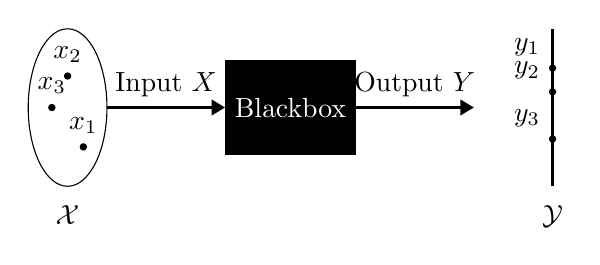
\begin{tikzpicture}[
 	node distance=5mm and 30mm,
	box/.style = {draw, minimum height=12mm, align=center},
	sx+/.style = {xshift= 15mm}, 
	sx-/.style = {xshift=-15mm},
	sx--/.style = {xshift=-20mm},
	sX--/.style = {xshift=-20mm,yshift=-1cm},
	sY--/.style = {xshift=25mm,yshift=-1cm},
	sx1--/.style = {xshift=-18mm,yshift=-5mm,},
	sx2--/.style = {xshift=-20mm,yshift=4mm},
	sx3--/.style = {xshift=-22mm,yshift=0mm},
	sxt++/.style = {xshift=25mm,yshift=1cm},
	sxb++/.style = {xshift=25mm,yshift=-1cm},
	sy1/.style = {xshift=25mm,yshift=5mm,},
	sy2/.style = {xshift=25mm,yshift=2mm},
	sy3/.style = {xshift=25mm,yshift=-4mm},
	every edge quotes/.style = {align=center},
	mycirc/.style={circle,fill=black, scale=.01cm}
     ]
		\node[fill=black,text=white] (n1) [box] {Blackbox};              
%
		\draw[thick,-Triangle]
		([sx-] n1.west) to [above,"Input $X$"] (n1.west);
%
		\draw[thick,-Triangle]
		(n1.east) to [above,"Output $Y$"] ([sx+] n1.east);
%
		\draw ([sx--] n1.west) ellipse (.5cm and 1cm);
		\node [mycirc,label=above:{$x_1$}] at ([sx1--] n1.west) {};
		\node [mycirc,label=above:{$x_2$}] at ([sx2--] n1.west) {};
		\node [mycirc,label=above:{$x_3$}] at ([sx3--] n1.west) {};
		\node [label=below:{$\mathcal{X}$}] at ([sX--] n1.west) {};
%
		\draw[thick,black] ([sxt++] n1.east) to ([sxb++] n1.east) ;
		\node [mycirc,label=above left:{$y_1$}] at ([sy1] n1.east) {};
		\node [mycirc,label=above left:{$y_2$}] at ([sy2] n1.east) {};
		\node [mycirc,label=above left:{$y_3$}] at ([sy3] n1.east) {};
		\node [label=below:{$\mathcal{Y}$}] at ([sY--] n1.east) {};
\end{tikzpicture}
\end{center}

Any fit parameters of predictions will be denoted by a hat $\hat{\theta}$. Assume we have come to a regression function by analyzing the training data $(x_i, y_i)$. The predicted output of the regression function will be denoted $\hat{Y}$. 
\end{frame}





\begin{frame}[fragile]{Inputs and Output}
\begin{center}
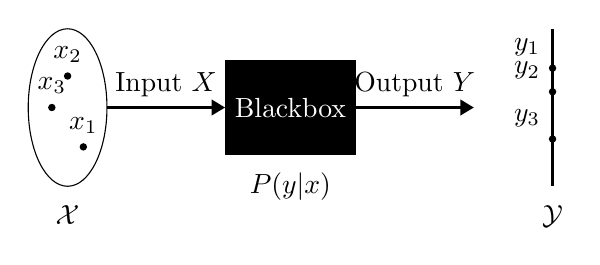
\begin{tikzpicture}[
 	node distance=5mm and 30mm,
	box/.style = {draw, minimum height=12mm, align=center},
	sx+/.style = {xshift= 15mm}, 
	sx-/.style = {xshift=-15mm},
	sx--/.style = {xshift=-20mm},
	sX--/.style = {xshift=-20mm,yshift=-1cm},
	sY--/.style = {xshift=25mm,yshift=-1cm},
	sV-/.style = {yshift=-1cm},
	sx1--/.style = {xshift=-18mm,yshift=-5mm,},
	sx2--/.style = {xshift=-20mm,yshift=4mm},
	sx3--/.style = {xshift=-22mm,yshift=0mm},
	sxt++/.style = {xshift=25mm,yshift=1cm},
	sxb++/.style = {xshift=25mm,yshift=-1cm},
	sy1/.style = {xshift=25mm,yshift=5mm,},
	sy2/.style = {xshift=25mm,yshift=2mm},
	sy3/.style = {xshift=25mm,yshift=-4mm},
	every edge quotes/.style = {align=center},
	mycirc/.style={circle,fill=black, scale=.01cm}
     ]
		\node[fill=black,text=white] (n1) [box] {Blackbox};  
		\node at ([sV-] n1) {$P(y|x)$};            
%
		\draw[thick,-Triangle]
		([sx-] n1.west) to [above,"Input $X$"] (n1.west);
%
		\draw[thick,-Triangle]
		(n1.east) to [above,"Output $Y$"] ([sx+] n1.east);
%
		\draw ([sx--] n1.west) ellipse (.5cm and 1cm);
		\node [mycirc,label=above:{$x_1$}] at ([sx1--] n1.west) {};
		\node [mycirc,label=above:{$x_2$}] at ([sx2--] n1.west) {};
		\node [mycirc,label=above:{$x_3$}] at ([sx3--] n1.west) {};
		\node [label=below:{$\mathcal{X}$}] at ([sX--] n1.west) {};
%
		\draw[thick,black] ([sxt++] n1.east) to ([sxb++] n1.east) ;
		\node [mycirc,label=above left:{$y_1$}] at ([sy1] n1.east) {};
		\node [mycirc,label=above left:{$y_2$}] at ([sy2] n1.east) {};
		\node [mycirc,label=above left:{$y_3$}] at ([sy3] n1.east) {};
		\node [label=below:{$\mathcal{Y}$}] at ([sY--] n1.east) {};
		
\end{tikzpicture}
\end{center}

\textbf{Goal Of Regression Analysis}: For any regression problem, we assume that there is an underlying true distribution of labels $P(Y|X)$ (read probability of $Y$ given $X$) that gives a probability (density) for any data point $X$ in the domain to have label $Y$. \pause We cant know $P$, we can only know the data drawn from it, but given that data we want to produce a fit distribution $\hat{P}(Y|X)$ that closely mimics $P$. 
\end{frame}



\begin{frame}[fragile]{Inputs and Output}
\begin{center}
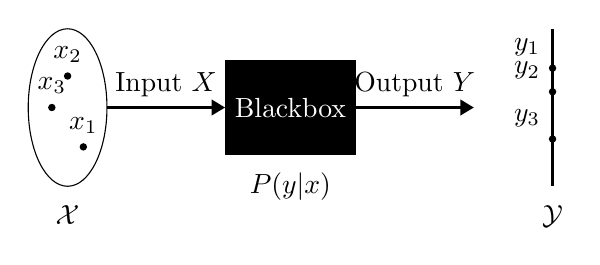
\begin{tikzpicture}[
 	node distance=5mm and 30mm,
	box/.style = {draw, minimum height=12mm, align=center},
	sx+/.style = {xshift= 15mm}, 
	sx-/.style = {xshift=-15mm},
	sx--/.style = {xshift=-20mm},
	sX--/.style = {xshift=-20mm,yshift=-1cm},
	sY--/.style = {xshift=25mm,yshift=-1cm},
	sV-/.style = {yshift=-1cm},
	sx1--/.style = {xshift=-18mm,yshift=-5mm,},
	sx2--/.style = {xshift=-20mm,yshift=4mm},
	sx3--/.style = {xshift=-22mm,yshift=0mm},
	sxt++/.style = {xshift=25mm,yshift=1cm},
	sxb++/.style = {xshift=25mm,yshift=-1cm},
	sy1/.style = {xshift=25mm,yshift=5mm,},
	sy2/.style = {xshift=25mm,yshift=2mm},
	sy3/.style = {xshift=25mm,yshift=-4mm},
	every edge quotes/.style = {align=center},
	mycirc/.style={circle,fill=black, scale=.01cm}
     ]
		\node[fill=black,text=white] (n1) [box] {Blackbox};  
		\node at ([sV-] n1) {$P(y|x)$};            
%
		\draw[thick,-Triangle]
		([sx-] n1.west) to [above,"Input $X$"] (n1.west);
%
		\draw[thick,-Triangle]
		(n1.east) to [above,"Output $Y$"] ([sx+] n1.east);
%
		\draw ([sx--] n1.west) ellipse (.5cm and 1cm);
		\node [mycirc,label=above:{$x_1$}] at ([sx1--] n1.west) {};
		\node [mycirc,label=above:{$x_2$}] at ([sx2--] n1.west) {};
		\node [mycirc,label=above:{$x_3$}] at ([sx3--] n1.west) {};
		\node [label=below:{$\mathcal{X}$}] at ([sX--] n1.west) {};
%
		\draw[thick,black] ([sxt++] n1.east) to ([sxb++] n1.east) ;
		\node [mycirc,label=above left:{$y_1$}] at ([sy1] n1.east) {};
		\node [mycirc,label=above left:{$y_2$}] at ([sy2] n1.east) {};
		\node [mycirc,label=above left:{$y_3$}] at ([sy3] n1.east) {};
		\node [label=below:{$\mathcal{Y}$}] at ([sY--] n1.east) {};
		
\end{tikzpicture}
\end{center}

\textbf{Goal Of Regression Analysis}: Produce a probability distribution $\hat{P}(Y|X)$ (read probability of $Y$ given $X$) that gives a probability (density) for any data point $x$ in the domain to have label $Y$. Usually, $\hat{P}(Y|X)$ is given by a function plus error $\hat{Y} = \hat{f}(X) + \epsilon$. 
\end{frame}




\begin{frame}[fragile]{Inputs and Output}

\textbf{Fitting the regression function}: The standard procedure for \textbf{fitting} a regression function is start with a \textbf{hypothesis class} of functions $\mathcal{H}$ that we will use for our model (e.g. linear functions, 2 layer perceptron networks, etc). We then define a loss function $L(y_i,  \hat{f}(x_i)) = L(y_i, \hat{y}_i)$ that gives the error between our prediction $\hat{y}_i$ and the actual label $y_i$. \pause

Formally, this paradigm of machine learning prescribes finding the $f\in \mathcal{H}$ that minimizes $\sum_i L(y_i, \hat{y}_i)$. The art of modern machine learning is in picking the hypothesis class, finding the minimum loss function within the hypothesis class, picking the loss function, and constructing more robust sets of samples. 
\end{frame}





\section{First Example: Linear Regression} 
\begin{frame}[fragile]{Linear Regression}
\textbf{The Problem:} Given a vector of inputs $X^T = (X_1,\ldots, X_p)$, we want to predict the output $Y$ via a linear model
$$
\hat Y = \hat\beta_0 + \sum_{j=1}^pX_j\hat\beta_j\,.
$$
The hats here denote fit constants. 

\pause

If we include a constant variable 1 in $X$ and write $\hat \beta = (\beta_0,\ldots, \beta_p)$, we can write
$$
\hat Y = \hat \beta^T X
$$
\end{frame}


\begin{frame}[fragile]{Linear Regression}
Note that $\hat Y$ need not be a scalar: if $\hat Y$ is a $K$ vector then $\hat \beta$ is an $p\times K$ matrix

\begin{align*}
\left[\begin{matrix}
\hat Y_1
\\
\vdots
\\
\hat Y_K
\end{matrix}\right]
&=
\left[\begin{matrix}
\hat \beta_{0,1}
\\
\vdots
\\
\hat \beta_{0,K}
\end{matrix}\right]
+
X_1\left[\begin{matrix}
\hat \beta_{1,1}
\\
\vdots
\\
\hat \beta_{1,K}
\end{matrix}\right]
+
\ldots
+
X_p
\left[\begin{matrix}
\hat \beta_{p,1}
\\
\vdots
\\
\hat \beta_{p,K}
\end{matrix}\right]
\\
\hat Y&= 
\left[\begin{matrix}
\hat \beta_{0,1}&\ldots &\hat \beta_{p,0}
\\
\vdots&\ddots&\vdots
\\
\hat \beta_{0,K} & \ldots & \hat \beta_{p,K}
\end{matrix}\right]
\left[\begin{matrix}
1\\
X_1\\
\vdots\\
X_p
\end{matrix}\right]
\\
\hat Y  &= \hat\beta^TX
\end{align*}

\end{frame}



\begin{frame}[fragile]{Linear Regression}
  \begin{minipage}[t][0.5\textheight][t]{\textwidth}
    \centering
     \includegraphics[height=0.5\textheight]{L1Regression1.png}
  \end{minipage}
  \vfill
  \begin{minipage}[t][0.5\textheight][t]{\textwidth}
How do we find $\hat\beta$ given a specific set of data? That is, how do we \textbf{fit} the linear model to data points $(x_i,y_i)$?
  \end{minipage}
\end{frame}



\begin{frame}[fragile]{Linear Regression}
  \begin{minipage}[t][0.5\textheight][t]{\textwidth}
    \centering
     \includegraphics[height=0.5\textheight]{L1Regression2.png}
  \end{minipage}
  \vfill
  \begin{minipage}[t][0.5\textheight][t]{\textwidth}
How do we find $\hat\beta$ given a specific set of data? That is, how do we \textbf{fit} the linear model to data points $(x_i,y_i)$?
  \end{minipage}
\end{frame}


\begin{frame}[fragile]{Linear Regression}
  \begin{minipage}[t][0.5\textheight][t]{\textwidth}
    \centering
     \includegraphics[height=0.5\textheight]{L1Regression3.png}
  \end{minipage}
  \vfill
  \begin{minipage}[t][0.5\textheight][t]{\textwidth}
How do we find $\hat\beta$ given a specific set of data? That is, how do we \textbf{fit} the linear model to data points $(x_i,y_i)$?
  \end{minipage}
\end{frame}



\begin{frame}[fragile]{Linear Regression}
  \begin{minipage}[t][0.5\textheight][t]{\textwidth}
    \centering
     \includegraphics[height=0.5\textheight]{L1Regression2.png}
  \end{minipage}
  \vfill
  \begin{minipage}[t][0.5\textheight][t]{\textwidth}
There are many ways. The most popular is by minimizing the \textbf{residual sum of squares} over the training set
$$
\text{RSS}(\beta) = \sum_{i=1}^N||y_i - \beta^T x_i||^2\,.
$$
  \end{minipage}
\end{frame}


\begin{frame}[fragile]{Linear Regression}
  \begin{minipage}[t][0.5\textheight][t]{\textwidth}
    \centering
     \includegraphics[height=0.5\textheight]{L1Regression4.png}
  \end{minipage}
  \vfill
  \begin{minipage}[t][0.5\textheight][t]{\textwidth}
There are many ways. The most popular is by minimizing the \textbf{residual sum of squares} over the training set. If $Y$ is a scalar,
$$
\text{RSS}(\beta) = \sum_{i=1}^N(y_i - \beta^T x_i)^2\,.
$$
  \end{minipage}
\end{frame}


\begin{frame}[fragile]{Linear Regression}
With a little bit of work, we can write
$$
\text{RSS}(\beta) = \sum_{i=1}^N(y_i - \beta^T x_i)^2
$$
in matrix form as
$$
\text{RSS}(\beta) = (\mathbf{y} - \mathbf{X}\beta)^T(\mathbf{y} - \mathbf{X}\beta)\,.
$$
\textbf{Proof:} First,  
$$
\mathbf{y} - \mathbf{X}\beta 
= 
\left[\begin{matrix}
y_1\\
\vdots\\
y_N
\end{matrix}\right]
-
\left[\begin{matrix}
-x_1-\\
\vdots\\
-x_N-
\end{matrix}\right]
\left[\begin{matrix}
\beta_0\\
\vdots\\
\beta_p
\end{matrix}\right]
=
\left[\begin{matrix}
y_1 - \beta^Tx_1\\
\vdots\\
y_N - \beta^Tx_N
\end{matrix}\right]\,.
$$
\end{frame}

\begin{frame}[fragile]{Linear Regression}
Then 
\begin{align*}
(\mathbf{y} - \mathbf{X}\beta)^T(\mathbf{y} - \mathbf{X}\beta) &= 
\left[\begin{matrix}
y_1 - \beta^Tx_1&
\ldots &
y_N - \beta^Tx_N
\end{matrix}\right]
\left[\begin{matrix}
y_1 - \beta^Tx_1\\
\vdots\\
y_N - \beta^Tx_N
\end{matrix}\right]
\\
&=
 \sum_{i=1}^N(y_i - \beta^T x_i)^2
\\
&=\text{RSS}(\beta) \,,
\end{align*}
as claimed.
\end{frame}




\begin{frame}[fragile]{Linear Regression}
Minimizing RSS($\beta$) becomes a problem of calculus. The minimum will occur when the partial derivatives are 0:
$$
0 = \frac{\partial}{\partial \beta_i} \text{RSS($\beta$)}\,.
$$
\pause
\textbf{Homework:} Show that the $p\times K$ derivatives 
$$
\frac{\partial}{\partial \beta} \text{RSS($\beta$)} := \frac{\partial}{\partial \beta_{ij}} \text{RSS($\beta$)}
$$
can be written compactly as
$$
\frac{\partial}{\partial \beta} \text{RSS($\beta$)} = -2\mathbf{X}^T(\mathbf{y} - \mathbf{X}\beta) \,.\pause
$$
Observe that this implies that $\frac{\partial}{\partial \beta} \text{RSS($\beta$)}  = 0$ when 
$$
\mathbf{X}^T(\mathbf{y} - \mathbf{X}\beta) = 0\,.
$$

\end{frame}




\begin{frame}[fragile]{Linear Regression}
  \begin{minipage}[t][0.5\textheight][t]{\textwidth}
    \centering
     \includegraphics[height=0.5\textheight]{L1Regression2.png}
  \end{minipage}
  \vfill
  \begin{minipage}[t][0.5\textheight][t]{\textwidth}
Solving $\mathbf{X}^T(\mathbf{y} - \mathbf{X}\beta) = 0$ for $\beta$ yields an explicit equation for the parameters
$$
\hat\beta = (\mathbf{X}^T\mathbf{X})^{-1}\mathbf{X}^T\mathbf{y}\,.
$$
It doesn't seem to take much data to get a decent answer here, but we do have to invert a matrix. The solution is also relatively \textbf{stable} - it would take the addition of many more data points to dramatically change it.
  \end{minipage}
\end{frame}




\section{Second Example: Binary Classification}


\begin{frame}[fragile]{Binary Classification}
  \begin{minipage}[t][0.5\textheight][t]{\textwidth}
    \centering
     \includegraphics[height=0.5\textheight]{L1BinaryClass1.png}
  \end{minipage}
  \vfill
  \begin{minipage}[t][0.5\textheight][t]{\textwidth}
We have here a scatter plot of two colored training data in $\mathcal{X} = \mathbb{R}^2$. The inputs are $X_1$ and $X_2$ and the outputs $Y$ take values in $\mathcal{G} = \{\text{Orange}, \text{Blue}\}$. 
  \end{minipage}
\end{frame}



\begin{frame}[fragile]{Binary Classification}
  \begin{minipage}[t][0.5\textheight][t]{\textwidth}
    \centering
     \includegraphics[height=0.5\textheight]{L1BinaryClass1.png}
  \end{minipage}
  \vfill
  \begin{minipage}[t][0.5\textheight][t]{\textwidth}
For any point $(X_1,X_2)$ we want to produce a probability $\hat Y$ that the point is labeled ``Orange" and probability $1-\hat{Y}$ that the point is labeled ``Blue."
  \end{minipage}
\end{frame}



\begin{frame}[fragile]{Binary Classification}
  \begin{minipage}[t][0.5\textheight][t]{\textwidth}
    \centering
     \includegraphics[height=0.5\textheight]{L1BinaryClass1.png}
  \end{minipage}
  \vfill
  \begin{minipage}[t][0.5\textheight][t]{\textwidth}

In the binary case, we may minimize $\text{RSS}(\beta)$ with $Y\in\{0,1\}$. We assign a color to $(X_1,X_2)$ by selecting
$$
\hat G = \begin{cases}
\text{Orange} & \text{if }\hat Y>.5
\\
\text{Blue} & \text{if }\hat Y\leq.5 
\end{cases}
$$

 \end{minipage}
\end{frame}


\begin{frame}[fragile]{Binary Classification}
  \begin{minipage}[t][0.5\textheight][t]{\textwidth}
    \centering
     \includegraphics[height=0.5\textheight]{L1BinaryClass2.png}
  \end{minipage}
  \vfill
  \begin{minipage}[t][0.5\textheight][t]{\textwidth}

In the binary case, we may minimize $\text{RSS}(\beta)$ with $Y\in\{0,1\}$. We assign a color to $(X_1,X_2)$ by selecting
$$
\hat G = \begin{cases}
\text{Orange} & \text{if }\hat Y>.5
\\
\text{Blue} & \text{if }\hat Y\leq.5 
\end{cases}
$$

 \end{minipage}
\end{frame}



\begin{frame}[fragile]{Binary Classification}
  \begin{minipage}[t][0.5\textheight][t]{\textwidth}
    \centering
     \includegraphics[height=0.5\textheight]{L1BinaryClass3.png}
  \end{minipage}
  \vfill
  \begin{minipage}[t][0.5\textheight][t]{\textwidth}

In this case, the two classes are separated by a linear \textbf{decision boundary} $\{x:\hat \beta x^T = .5\}$.\newline

\textbf{Question:} What do you think of this model? How could it be improved? Can we minimize the apparent errors?

 \end{minipage}
\end{frame}



\begin{frame}[fragile]{Binary Classification}
  \begin{minipage}[t][0.5\textheight][t]{\textwidth}
    \centering
     \includegraphics[height=0.5\textheight]{L1BinaryClass3.png}
  \end{minipage}
  \vfill
  \begin{minipage}[t][0.5\textheight][t]{\textwidth}

The theoretical accuracy of the linear classifier will depend on the mechanism of data generation. Consider the following two cases:

\textbf{Scenario 1:} The data was generated from a pair of multivariate normal distributions with different means.

\textbf{Scenario 2:} The data was generated from many low variance distributions with normally distributed means.


 \end{minipage}
\end{frame}



\begin{frame}[fragile]{Binary Classification}
  \begin{minipage}[t][0.5\textheight][t]{\textwidth}
    \centering
     \includegraphics[height=0.5\textheight]{L1PairOfGuassians.png}
  \end{minipage}
  \vfill
  \begin{minipage}[t][0.5\textheight][t]{\textwidth}


\textbf{Scenario 1:} If data was generated from a pair of multivariate normal distributions with different means, the linear classifier might be the best we can do. 


 \end{minipage}
\end{frame}



\begin{frame}[fragile]{Binary Classification}
  \begin{minipage}[t][0.5\textheight][t]{\textwidth}
    \centering
     \includegraphics[height=0.5\textheight]{L1BinaryClass7.png}
  \end{minipage}
  \vfill
  \begin{minipage}[t][0.5\textheight][t]{\textwidth}


\textbf{Scenario 2:} If data was generated from many low variance distributions with normally distributed means, then the best classifier requires a much more nuanced approach.

 \end{minipage}
\end{frame}




\begin{frame}[fragile]{Binary Classification}
  \begin{minipage}[t][0.5\textheight][t]{\textwidth}
    \centering
     \includegraphics[height=0.5\textheight]{L1BinaryClass6.png}
  \end{minipage}
  \vfill
  \begin{minipage}[t][0.5\textheight][t]{\textwidth}


\textbf{Scenario 2:} If data was generated from many low variance distributions with normally distributed means, then the best classifier requires a much more nuanced approach.

 \end{minipage}
\end{frame}




\begin{frame}[fragile]{Binary Classification}
  \begin{minipage}[t][0.5\textheight][t]{\textwidth}
    \centering
     \includegraphics[height=0.5\textheight]{L1BinaryClass5.png}
  \end{minipage}
  \vfill
  \begin{minipage}[t][0.5\textheight][t]{\textwidth}


\textbf{Scenario 2:} If data was generated from many low variance distributions with normally distributed means, then the best classifier would have a much more complicated boundary than a simple line, and may not be connected. 

 \end{minipage}
\end{frame}






\begin{frame}[fragile]{Binary Classification: Nearest Neighbors}
  \begin{minipage}[t][0.5\textheight][t]{\textwidth}
    \centering
     \includegraphics[height=0.5\textheight]{L1BinaryClass1.png}
  \end{minipage}
  \vfill
  \begin{minipage}[t][0.5\textheight][t]{\textwidth}

One way to complicate the boundary is the \textbf{$\mathbf k$-nearest neighbors} method. For any pair of input values $X$, we determine a labeling by
$$
\hat Y(x) = \frac{1}{k}\sum_{x_i\in N_k(x)}y_i \,,
$$
where $N_k(x)$ are the $k$ points in the training set closest to $x$. 


 \end{minipage}
\end{frame}




\begin{frame}[fragile]{Binary Classification: Nearest Neighbors}
  \begin{minipage}[t][0.5\textheight][t]{\textwidth}
    \centering
     \includegraphics[height=0.5\textheight]{L1KNN1.png}
  \end{minipage}
  \vfill
  \begin{minipage}[t][0.5\textheight][t]{\textwidth}

One way to complicate the boundary is the \textbf{$\mathbf k$-nearest neighbors} method. For any pair of input values $X$, we determine a labeling by
$$
\hat Y(x) = \frac{1}{k}\sum_{x_i\in N_k(x)}y_i \,,
$$
where $N_k(x)$ are the $k$ points in the training set closest to $x$. 
 \end{minipage}
\end{frame}


\begin{frame}[fragile]{Binary Classification: Nearest Neighbors}
  \begin{minipage}[t][0.5\textheight][t]{\textwidth}
    \centering
     \includegraphics[height=.5\textheight]{L1KNN1.png}
  \end{minipage}
  \vfill
  \begin{minipage}[t][0.5\textheight][t]{\textwidth}

Notice that the boundary is much more jagged in this case, but we also have fewer misclassifications of the training data. Such misclassifications are can be expressed as the \textbf{training error}. 

The training error is roughly an increasing function of $k$. When $k=1$ the training error is 0. When $k = N$ the training error is roughly 50\% (assuming equal number of each label).
 \end{minipage}
\end{frame}


\begin{frame}[fragile]{Binary Classification: Nearest Neighbors}
  \begin{minipage}[t][0.5\textheight][t]{\textwidth}
    \centering
     \includegraphics[height=0.5\textheight]{L1KNN2.png}
  \end{minipage}
  \vfill
  \begin{minipage}[t][0.5\textheight][t]{\textwidth}
$$
\mathbf{k=1}
$$

When $k=1$ the training error is 0. When $k = N$ the training error is roughly 50\%.  
 \end{minipage}
\end{frame}



\begin{frame}[fragile]{Binary Classification: Nearest Neighbors}
  \begin{minipage}[t][0.5\textheight][t]{\textwidth}
    \centering
     \includegraphics[height=0.5\textheight]{L1KNN1.png}
  \end{minipage}
  \vfill
  \begin{minipage}[t][0.5\textheight][t]{\textwidth}
$$
\mathbf{k=10}
$$

When $k=1$ the training error is 0. When $k = N$ the training error is roughly 50\%.  
 \end{minipage}
\end{frame}



\begin{frame}[fragile]{Binary Classification: Nearest Neighbors}
  \begin{minipage}[t][0.5\textheight][t]{\textwidth}
    \centering
     \includegraphics[height=0.5\textheight]{L1KNN3.png}
  \end{minipage}
  \vfill
  \begin{minipage}[t][0.5\textheight][t]{\textwidth}
$$
\mathbf{k=50}
$$

When $k=1$ the training error is 0. When $k = N$ the training error is roughly 50\%.  
 \end{minipage}
\end{frame}


\begin{frame}[fragile]{Binary Classification: Nearest Neighbors}
  \begin{minipage}[t][0.5\textheight][t]{\textwidth}
    \centering
     \includegraphics[height=0.5\textheight]{L1KNN4.png}
  \end{minipage}
  \vfill
  \begin{minipage}[t][0.5\textheight][t]{\textwidth}
$$
\mathbf{k=100}
$$

When $k=1$ the training error is 0. When $k = N$ the training error is roughly 50\%.  
 \end{minipage}
\end{frame}


\begin{frame}[fragile]{Binary Classification: Nearest Neighbors}
  \begin{minipage}[t][0.5\textheight][t]{\textwidth}
    \centering
     \includegraphics[height=0.5\textheight]{L1KNN4.png}
  \end{minipage}
  \vfill
  \begin{minipage}[t][0.5\textheight][t]{\textwidth}
$$
\mathbf{k=100}
$$

Note: It appears that $k$-nearest neighbors has a single parameter $k$, but we can't fit this parameter using lease squares since we will always just get $k=1$. 
 \end{minipage}
\end{frame}




\begin{frame}[fragile]{Binary Classification: Comparison}
  \begin{minipage}[t][0.7\textheight][t]{\textwidth}
    \centering
     \includegraphics[height=0.7\textheight]{L1LinearVsKNN.png}
  \end{minipage}
  \vfill
  \begin{minipage}[t][0.3\textheight][t]{\textwidth}
Comparing the linear model to the $k$-nearest neighbors, we see that while the training error decreases as $N/k$ increases, the true error is relatively high on both ends. 
 \end{minipage}
\end{frame}






\section{Course Structure and Policies}

\begin{frame}[fragile]{Course Texts}
This course will follow a pair a text books:

\begin{itemize}[label={}]
\item \textbf{High level:} \textit{The Elements of Statstical Learning}. Trevor Hastie Robert Tibshirani, Jerome Friedman. 

\item \textbf{Low level:} \textit{Understanding Machine Learning: From Theory to Algorithms}. Shai Shalev-Shwartz, Shai Ben-David.

\end{itemize}

There is also a practicum book which is worth having if you're interested in machine learning:

\begin{itemize}[label={}]
\item \textbf{Implementation:} \textit{Hands-On Machine Learning with Scikit-Learn and TensorFlow: Concepts, Tools, and Techniques to Build Intelligent Systems}. Aurélien Géron. 
\end{itemize}

Society and impact:

\begin{itemize}[label={}]
\item \textbf{Implementation:} \textit{Weapons of math destruction}. Cathy O'Neil.
\end{itemize}
\end{frame}





\begin{frame}[fragile]{Course Policies}
The course grade will be divided up as follows:

30\% Homework

30\% Labs

40\% Final Project
\end{frame}



\begin{frame}[fragile]{Homework}
Homeworks will be due Tuesday in class in weeks 3, 5 and 7. You are free to discuss homework with me in office hours. You may work in study groups, but all work turned in must be your own. Homework will be partially graded on presentation, and extra points will be awarded for homework completed in latex. 
\end{frame}




\begin{frame}[fragile]{Labs}
Labs will use Python and will be distributed as Jupyter Notebooks. They will be turned in through Blackboard. There will be roughly 6 labs beginning in week 4. The labs will be partially in class, and should take no longer than the allotted class time in theory, but extra credit will be given for going above and beyond, both in presentation and in results. 
\end{frame}




\section{Final Project}

\begin{frame}[fragile]{Project}
The final project will consist of a project report (roughly 5 pages) and presentation (roughly 10 minutes). \pause

Project groups should contain 2-4 people.\pause

Projects can be of one of three forms: \pause
\begin{itemize}
\item A computational analysis of a data set using sufficiently complicated or novel techniques from this course.
\item A theoretical presentation of a topic not covered in this course with a case study.
\item Machine learning project from external source (industry, PhD work, etc)
\end{itemize}
I am more than happy to discuss possible projects in any of these categories with you.
\end{frame}




\begin{frame}[fragile]{Automatic segmentation tool for medical imaging }
  \begin{minipage}[t][0.5\textheight][t]{\textwidth}
	\centering \includegraphics[height=0.5\textheight]{168927158.png} 
  \end{minipage}
  \vfill
\begin{minipage}[t][0.5\textheight][t]{\textwidth}
This project would involve taking stacks of 2d MRI data and segmenting it to pull out 3d features. The goal of the project is to eventually register the 3d images with depth scans (video) of patients heads, so that a surgeon can see a patients head with the volumetric features from the MRI super imposed. 
\end{minipage}
\end{frame}



\begin{frame}[fragile]{Automatic segmentation tool for medical imaging }
  \begin{minipage}[t][0.5\textheight][t]{\textwidth}
	\centering \includegraphics[height=0.5\textheight]{VoxelSlice.png} 
  \end{minipage}
  \vfill
\begin{minipage}[t][0.5\textheight][t]{\textwidth}
Training data will be a set of MRI scans from patients in one of three stages of dementia. The task will be to train a volumetric convolutional net that can classify a scan into the stages of dementia. The OASIS 1 dataset contains 416 volumetric MRI images at 12 MB each, or around 5 Gb of data. 
\end{minipage}
\end{frame}






\begin{frame}[fragile]{Automatic segmentation tool for medical imaging }
Initially, it will be a simple classification project. Using the OASIS (Open Axis Series of Imaging Studies) 1 MRI dataset, you will try to classify MRI scans as coming from the brain of a patient diagnosed with dementia. \pause

I will provide a 2d sampling of data containing around 600 images, your first attempts at classification will be from that dataset. As the semester goes on, you should expect to use the tools presented to try to improve your fit, and eventually to use a full 3d convolutional neural network to fit the data. \pause

There is a lot of room in this project to pick up soft skills like git, AWS, and Google Cloud. Groups are recommended to heavily delegate and work together across groups. \pause

The 2D images dataset has been posted on blackboard and will be incorporated into some of the labs. 
\end{frame}




\begin{frame}[fragile]{Project}
Rough timeline: 
\begin{itemize}
\item Group Selection: January 27
\item Project Proposal Deadline: February 3
\item Progress Report: February 24
\item First Draft: March 16
\item Final Draft: April 6
\item Presentations: April 13 - 24.
\end{itemize}
These may change depending on the loss function.
\end{frame}


\subsection{Projects}
\subsection{Resources}


\end{document}